\section{Verteilte Systeme}

\begin{definition}{Verteiltes System}\\
Ein Netzwerk aus autonomen Computern und Softwarekomponenten, die als einheitliches System erscheinen:
\begin{itemize}
    \item Autonome Knoten und Komponenten
    \item Netzwerkverbindung
    \item Erscheint als ein System
\end{itemize}
\end{definition}

\begin{concept}{Charakteristika verteilter Systeme}\\
Typische Merkmale moderner verteilter Systeme:
\begin{itemize}
    \item \textbf{Skalierbarkeit:} Oft sehr große Systeme
    \item \textbf{Datenorientierung:} Zentrale Datenbanken
    \item \textbf{Interaktivität:} GUI und Batch-Verarbeitung
    \item \textbf{Nebenläufigkeit:} Parallele Benutzerinteraktionen
    \item \textbf{Konsistenz:} Hohe Anforderungen an Datenkonsistenz
\end{itemize}
\end{concept}

\begin{theorem}{Grundlegende Konzepte}\\
\textbf{1. Kommunikation:}
\begin{itemize}
    \item Remote Procedure Calls (RPC)
    \item Message Queuing
    \item Publish-Subscribe-Systeme
\end{itemize}

\textbf{2. Fehlertoleranz:}
\begin{itemize}
    \item Replikation von Komponenten
    \item Failover-Mechanismen
    \item Fehlererkennung und -behandlung
\end{itemize}

\textbf{3. Fehlersemantik:}
\begin{itemize}
    \item Konsistenzgarantien
    \item Recovery-Verfahren
    \item Kompensationsmechanismen
\end{itemize}
\end{theorem}

\begin{concept}{Architekturmuster}\\
Grundlegende Architekturstile für verteilte Systeme:
\begin{itemize}
    \item \textbf{Client-Server:} Zentraler Server, multiple Clients
    \item \textbf{Peer-to-Peer:} Gleichberechtigte Knoten
    \item \textbf{Publish-Subscribe:} Event-basierte Kommunikation
\end{itemize}
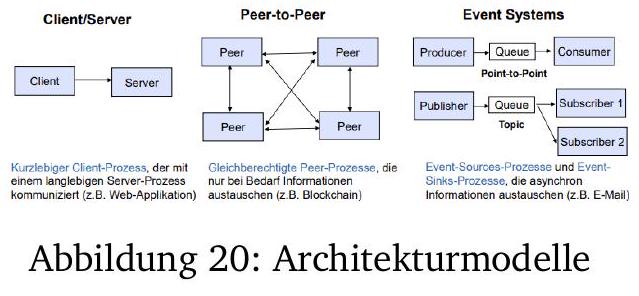
\includegraphics[width=0.9\linewidth]{images/2024_12_29_0d1d7b5551ea1b4b41bdg-18}
\end{concept}

\begin{KR}{Entwurf verteilter Systeme}\\
\textbf{1. Systemanalyse}
\begin{itemize}
    \item Anforderungen identifizieren
    \item Verteilungsaspekte analysieren
    \item Konsistenzanforderungen definieren
\end{itemize}

\textbf{2. Architekturentscheidungen}
\begin{itemize}
    \item Architekturstil wählen
    \item Kommunikationsmuster festlegen
    \item Fehlertoleranzstrategie definieren
\end{itemize}

\textbf{3. Technologieauswahl}
\begin{itemize}
    \item Middleware evaluieren
    \item Protokolle bestimmen
    \item Werkzeuge auswählen
\end{itemize}
\end{KR}

\begin{concept}{Middleware-Technologien}\\
Gängige Technologien für verteilte Systeme:
\begin{itemize}
    \item \textbf{Message Broker:} 
    \begin{itemize}
        \item Apache Kafka
        \item RabbitMQ
    \end{itemize}
    \item \textbf{RPC Frameworks:}
    \begin{itemize}
        \item gRPC
        \item CORBA
    \end{itemize}
    \item \textbf{Web Services:}
    \begin{itemize}
        \item RESTful APIs
        \item GraphQL
    \end{itemize}
\end{itemize}
\end{concept}

\begin{example}{Client-Server Implementation}\\
\textbf{Aufgabe:} Implementieren Sie einen einfachen Echo-Server mit Java.

\textbf{Lösung:}
\begin{lstlisting}[language=Java, style=base]
// Server
public class EchoServer {
    public static void main(String[] args) {
        try (ServerSocket server = new ServerSocket(8080)) {
            while (true) {
                Socket client = server.accept();
                new Thread(() -> handleClient(client)).start();
            }
        }
    }
    
    private static void handleClient(Socket client) {
        try (
            BufferedReader in = new BufferedReader(
                new InputStreamReader(client.getInputStream()));
            PrintWriter out = new PrintWriter(
                client.getOutputStream(), true)
        ) {
            String line;
            while ((line = in.readLine()) != null) {
                out.println("Echo: " + line);
            }
        } catch (IOException e) {
            e.printStackTrace();
        }
    }
}

// Client
public class EchoClient {
    public static void main(String[] args) {
        try (
            Socket socket = new Socket("localhost", 8080);
            PrintWriter out = new PrintWriter(
                socket.getOutputStream(), true);
            BufferedReader in = new BufferedReader(
                new InputStreamReader(socket.getInputStream()))
        ) {
            out.println("Hello Server!");
            System.out.println(in.readLine());
        } catch (IOException e) {
            e.printStackTrace();
        }
    }
}
\end{lstlisting}
\end{example}

\begin{example}{Publish-Subscribe Pattern}\\
\textbf{Aufgabe:} Implementieren Sie ein einfaches Event-System.

\textbf{Lösung:}
\begin{lstlisting}[language=Java, style=base]
public class EventBus {
    private Map<String, List<EventHandler>> handlers = new HashMap<>();
    
    public void subscribe(String event, EventHandler handler) {
        handlers.computeIfAbsent(event, k -> new ArrayList<>())
               .add(handler);
    }
    
    public void publish(String event, String data) {
        if (handlers.containsKey(event)) {
            handlers.get(event)
                   .forEach(handler -> handler.handle(data));
        }
    }
}

interface EventHandler {
    void handle(String data);
}

// Verwendung
EventBus bus = new EventBus();
bus.subscribe("userLogin", data -> 
    System.out.println("User logged in: " + data));
bus.publish("userLogin", "john_doe");
\end{lstlisting}
\end{example}

\begin{KR}{Typische Fehlerquellen}\\
\textbf{1. Netzwerkfehler}
\begin{itemize}
    \item Verbindungsabbrüche
    \item Timeouts
    \item Partitionierung
\end{itemize}

\textbf{2. Konsistenzprobleme}
\begin{itemize}
    \item Race Conditions
    \item Veraltete Daten
    \item Lost Updates
\end{itemize}

\textbf{3. Skalierungsprobleme}
\begin{itemize}
    \item Lastverteilung
    \item Resource-Management
    \item Bottlenecks
\end{itemize}

\textbf{Lösungsstrategien:}
\begin{itemize}
    \item Circuit Breaker Pattern
    \item Retry mit Exponential Backoff
    \item Idempotente Operationen
    \item Optimistic Locking
\end{itemize}
\end{KR}
